\section{时序超图存储结构和查询引擎}
时序超图存储的设计思路与时序RDF图存储类似,都使用了分布式键值存储辅以分布式排序数组的存储结构。时序超图查询引擎使用存储层提供的接口逐一执行HQL-T查询语句中的各RP。本节将详细介绍时序超图的存储结构和查询引擎。
\subsection{存储结构}
\label{sec:hyperstore}
系统支持的时序超图数据集格式为\texttt{时序超边类型,时序超边名称,有效时间区间的开始时间,有效时间区间的截止时间,\{顶点名称1,顶点名称2,...\}}。
\sys 同样会将时序超图数据集中的字符串转化成整型ID进行存储。系统默认使用32位UINT表示顶点字符串对应的ID(下称\texttt{vid}),取值范围为$[2^{16}, 2^{32})$,对于顶点数量比较庞大的数据集,可以在系统编译时指定使用64位UINT表示\texttt{vid},取值范围就扩充到$[2^{16}, 2^{48})$。系统使用64位UINT表示时序超边ID(下称\texttt{heid}),取值范围为$[2^{16}, 2^{48})$。值得注意的是,可能有多条时序超边的名称相同,例如字符串“群聊1”可能对应多条时序超边,表示“群聊1”在不同时间区间下的成员情况。系统会给予相同名称的不同时序超边不同的\texttt{heid},在将表示时序超边名称的字符串转换成\texttt{heid}时,字符串服务器返回的是\texttt{heid}的列表。表示时序超边和顶点的类型的字符串对应的ID(下分别称\texttt{htid}和\texttt{tid})的范围为$[2,2^{16})$。

时序超图存储内存布局如图\ref{thyperstore},与时序RDF图存储类似,它分为键值存储区和时序超边存储区两部分。
时序超边存储区存储的是每个超边的ID、类型及其有效时间,即由\texttt{
[超边ID,超边类型,有效时间区间的开始时间,有效时间区间的截止时间]}四元组组成,它本质上也是内存数组。时序超边存储区分为两部分,在“时序超边存储1”中,四元组按照有效时间区间的开始时间升序排布;在“时序超边存储2”中,四元组按照有效时间区间的截止时间升序排布。时序超边的\texttt{heid}与它对应的四元组在“时序超边存储1”中的偏移量\texttt{off}的关系为:
\begin{equation}
    \mathtt{heid = off + 2^{16}}
\end{equation}
键值存储区中的键值对分为直接索引和间接索引两类,在直接索引中,值是实际数据;在间接索引中,值由指向“时序超边存储1”中四元组的指针组成。

\begin{figure}[!htb]
\center{
\includegraphics[width=0.6\textwidth]  {figures/thyperstore.eps}}
\bicaption{时序超图存储内存布局}{Temporal hypergraph storage memory layout}
\label{thyperstore}
\end{figure}

在键值存储区中,各种键值对及其类型如表\ref{tab:thyper}所示,系统使用两个分布式键值存储结构V2E KV和E2V KV来存储这些键值对。
键值对\ding{182}\textasciitilde\ding{184}位于E2V KV,键的数据类型是64位UINT,值的基本数据类型和\texttt{vid}的数据类型相同;键值对\ding{185}\textasciitilde\ding{188}位于V2E KV,键的数据类型也是64位UINT,由高48位和低16位两部分组成,值的基本数据类型是64位UINT。E2V KV中的键值对都是直接索引,V2E KV中的键值对除了\ding{185}外都是间接索引。
\begin{table}[!hpt]
  \bicaption{时序超图存储使用的键值对}{Key-value pairs used in temporal hypergraph storage}
  \label{tab:thyper}
  \centering
  \begin{tabular}{p{1cm}p{2cm}p{8cm}p{3cm}} \toprule
    序号 & 键 & 值 & 类型 \\ \midrule
    \ding{182}\centering & \texttt{[htid]} & 类型为\texttt{htid}的所有时序超边包含的所有\texttt{vid} & \multirow{4}{*}{直接索引} \\
    \ding{183}\centering & \texttt{[tid]} & 类型为\texttt{tid}的所有\texttt{vid} & \\
    \ding{184}\centering & \texttt{[heid]} & 时序超边\texttt{heid}包含的所有\texttt{vid} & \\
    \ding{185}\centering & \texttt{[vid|0]} & 顶点\texttt{vid}的\texttt{tid} & \\ 
    \hline
    \ding{186}\centering & \texttt{[vid|htid]} & 包含顶点\texttt{vid}且类型为\texttt{htid}的所有时序超边 & \multirow{2}{*}{间接索引} \\ 
    \ding{187}\centering & \texttt{[0|htid]} & 类型为\texttt{htid}的所有时序超边 & \\ 
    \bottomrule
  \end{tabular}
\end{table}

图\ref{thsdemo}(a)展示了一个简单的时序超图拓扑,它从微信中的群聊及公众号和微信用户之间的关系抽象而来,它包含两类时序超边:群聊成员和公众号关注者。
有两条类型为群聊成员的时序超边:“群聊1”、“群聊2”,有三条类型为公众号关注者的时序超边:“公众号1”、“公众号2”、“公众号3”,有10个名称分别为A\textasciitilde J的类型为微信用户的顶点。
图\ref{thsdemo}(b)给出了系统会为其生成的一部分键值对。为了便于理解,图中使用字符串表示时序超边、顶点及其类型,系统实际使用的是这些字符串对应的ID。
在间接索引中,值是一个由时序超边对应的四元组在“时序超边存储1”中的偏移量组成的列表,例如,时序超边“群聊2”对应的四元组在“时序超边存储1”中的偏移量为1,那么间接索引就使用1来表示“群聊2”。

\begin{figure}[!htb]
\center{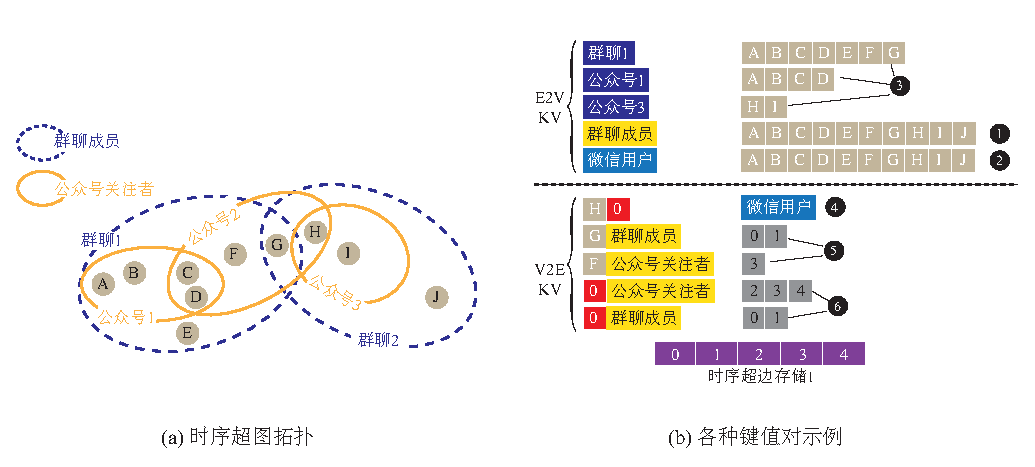
\includegraphics[width=0.95\textwidth]  {figures/thsdemo.eps}}
\bicaption{时序超图存储使用的键值对示例}{Example of key-value pairs used in temporal hypergraph storage}
\label{thsdemo}
\end{figure}

为了实现分布式可扩展存储,系统使用如下规则将键值对和时序超边划分到各查询节点中存储:
\begin{enumerate}
    \item \label{partitionRule1} 每个查询节点负责一块连续ID的时序超边和顶点的管理,时序超边\texttt{heid}会被分配到的查询节点(查询节点从0开始编号)为:
    \begin{equation}
        \mathtt{(heid - 2^{16}) \ / \ \lceil num\_thes \ / \ num\_qnodes \rceil}
    \end{equation}
    其中\texttt{num\_thes}是时序超边总数,\texttt{num\_qnodes}是查询节点数。顶点的分配方法同理。
    \item 对于键值对\ding{182}\ding{183}\ding{187},将值按照\ref{partitionRule1}中的规则划分到各查询节点存储,同一键会出现在每个查询节点的键值存储中;对于键值对\ding{184}\ding{185}\ding{186},将键依据其高48位按照\ref{partitionRule1}中的规则划分到不同查询节点存储,每个键只会出现在一个查询节点的键值存储中。
    \item 将所有四元组分别按有效时间区间的开始时间和截止时间排序后,分别按块划分到各查询节点的“时序超边存储1”和“时序超边存储2”中存储,偏移量为\texttt{off}的四元组会被分配到的查询节点(从0开始编号)为:
    \begin{equation}
        \mathtt{off \ / \ \lceil num\_thes \ / \ num\_qnodes \rceil}
    \end{equation}
\end{enumerate}

\subsection{查询引擎}
HQL-T查询引擎同样沿用了Wukong使用的图探索和全历史剪枝算法。默认情况下,查询引擎会使用存储层提供的接口通过键值存储查找所需的数据,但对于一些以时间点或时间范围为条件的查询,直接在“时序超边存储”上通过二分法查找符合条件的时序超边可能更加高效。例如图\ref{hql}中的查询语句是要查找最后一次成员变动发生于2023年10月1日到2023年10月7日期间的所有群聊及其成员,在执行该语句时,可以使用“时序超边存储1”快速找到有效时间区间开始时间在2023年10月1日到2023年10月7日期间的所有时序超边,然后从中筛选出类型为“群聊成员”且有效时间区间截止时间晚于当前时间的时序超边即可。如果查询引擎不使用“时序超边存储”,而是先从键值存储中找到所有类型为“群聊成员”的时序超边,再筛选出有效时间区间符合条件的时序超边,那么就会带来更大的数据访问开销。目前系统尚未实现HQL-T的查询优化器,无法自动判断使用键值存储和使用“时序超边存储”哪个效率更高。系统的替代方案是将选择权交给用户,由用户在查询语句中使用\textbf{时序超边时间范围模式}显式地指定使用“时序超边存储”进行时间条件查询,语法为:
\begin{equation}
    \mathtt{?var \ STRAT/END(const_1, const_2) \ interval}
\end{equation}

其中变量\texttt{?var}会取值为查询到的时序超边的\texttt{heid};\texttt{START}和\texttt{END}二选一,\texttt{START}指定依据有效时间区间开始时间进行查找,\texttt{END}指定依据有效时间区间截止时间进行查找;\texttt{const$_1$}和\texttt{const$_2$}是两个时间常量且\texttt{const$_1\leq$const$_2$},用于指定要查找的时间范围;\texttt{interval}是可选的,它是一个由两个变量组成的区间,格式为\texttt{[?var$_1$,?var$_2$)},当它存在时,两个变量会分别取值为查询到的时序超边的有效时间区间的开始时间和截止时间。我们规定,时序超边时间范围模式只能出现在GP中最开始的位置,它们会先于RP被处理。值得注意的是,用户需要自行估算使用时序超边时间范围模式是否能够提高查询的执行效率,避免出现负优化。图\ref{guide}中的查询语句与图\ref{hql}中的查询语句含义相同,但它显式地指定使用“时序超边存储1”进行时间范围查询。

\begin{figure}[!htb]
\center{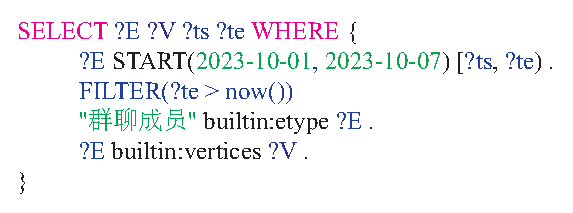
\includegraphics[width=0.55\textwidth]  {figures/guide.eps}}
\bicaption{显式指定使用“时序超边存储”的查询语句示例}{Example of a query that explicitly specifies the use of "temporal hyperedge storage"}
\label{guide}
\end{figure}

与SPARQL-T类似,HQL-T查询语句同样可分为大查询和小查询两类,大查询通常以大量时序超边或顶点作为起始,然后探索更多数量的时序超边和顶点;小查询通常从一个固定的时序超边或顶点开始,访问少量的时序超边和顶点。具体来说,大查询包含以下两类:
\begin{enumerate}
    \item 第一个查询模式是GE或GV模式的查询语句;
    \item 包含时序超边时间范围模式的查询语句。
\end{enumerate}
其他的查询语句都属于小查询。
查询引擎同样使用fork-join机制来处理大查询,其过程与SPARQL-T查询引擎完全相同,在此不作赘述。

查询引擎在处理小查询时同样可能会使用fork-join机制:当工作线程在准备开始执行一个RP时,如果中间结果条目数达到系统预设的阈值(例如100),且工作线程需要通过较多跨节点的单边RDMA Read操作来执行该RP,那么工作线程会将其分成\texttt{num\_qnodes}个子查询,然后分别发送给各个查询节点的一个工作线程共同执行。在划分查询时,中间结果是依据输入元素列表中的第一个变量的取值划分的,如果某行中间结果中该变量的取值为\texttt{val},那么该行中间结果会被划分到的子查询(从0开始编号)为:
\begin{equation}
    \mathtt{(val - 2^{16}) \ / \ \lceil num\_thes \ / \ num\_qnodes \rceil}
\end{equation}

V2E、E2V、V2V和E2E这四种RP的执行比较复杂,执行这些模式时输入元素列表中各变量的状态一定是Known,输出元素列表中变量的状态是Known或Unknown。接下来我们分别详细介绍这四种RP的执行逻辑,我们只讨论输出元素列表中变量的状态是Unknown的情况;对于V2E、E2V和E2E模式,我们只讨论包含\texttt{interval}的情况。
\begin{itemize}
    \item \textbf{V2E模式:}该模式的输入元素列表可以包含若干表示顶点的常量或变量。执行该模式时,首先需要使用键值对\ding{186}分别获取输入元素列表中的各常量对应的\texttt{heid}集合,然后求取这些集合的交集$s_1$。接下来对于每行中间结果,再使用键值对\ding{186}分别获取输入元素列表中各变量取值对应的\texttt{heid}集合,求取这些集合的交集$s_2$,然后求取$s_1$和$s_2$的交集$s$,$s$即是该变量可取值的集合。最后根据\texttt{heid}计算出偏移量,在“时序超边存储1”中读取对应四元组中的生命周期信息即可。
    \item \textbf{E2V模式:}该模式的输入元素列表可以包含若干表示时序超边的常量或变量。输入元素列表中的一个常量可能对应多条时序超边,查询引擎需要首先计算能够使得每个常量对应的时序超边都有且仅有一个有效的所有时间区间,记为$itv_1, itv_2,...,itv_n$(在图\ref{e2v}中是红色虚线标出的三个时间区间),然后对于每一个时间区间,使用键值对\ding{184}分别获取每条有效的时序超边对应的\texttt{vid}集合并求交集,记得到的集合为$s_1, s_2, ..., s_n$。接下来对于每行中间结果,计算能够使得输入元素列表中各变量取值表示的时序超边都有效的最大时间区间,记为$itv$(在图\ref{e2v}中是黑色虚线标出的时间区间,由于每个变量的取值只能表示一条时序超边,所以此处最多计算得到一个时间区间),然后使用键值对\ding{184}分别获取这些时序超边对应的\texttt{vid}集合,求取这些集合的交集$s$,最后将时间区间$itv$分别与时间区间$itv_1, itv_2,...,itv_n$求交,得到新的时间区间$itv_1', itv_2',...,itv_m'$(在图\ref{e2v}中是黑色双向箭头标出的两个时间区间)并计算每个新时间区间上$s_i$和$s$的交集$s_i'$。最终,一行中间结果能够生成$|s_1'|+|s_2'|+...+|s_m'|$行新的中间结果。
    
    \begin{figure}[!htb]
    \center{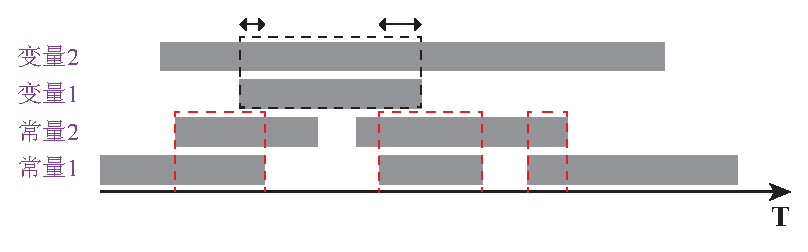
\includegraphics[width=0.6\textwidth]  {figures/e2v.eps}}
    \bicaption{执行E2V模式时对时间区间的处理过程}{Processing of time intervals when executing E2V pattern}
    \label{e2v}
    \end{figure}
    
    \item \textbf{V2V模式:}该模式的输入元素列表可以包含若干表示顶点的常量或变量。执行该模式时,首先要为输出元素列表中的变量寻找候选取值,为此,查询引擎将包含输入元素列表中第一个常量(如果输入元素列表没有常量,则是第一个变量的取值)所表示的顶点的所有时序超边包含的所有顶点作为候选顶点集合。确定候选顶点集合后,查询引擎会逐一验证每个候选顶点是否同时与各输入顶点出现在相同时序超边且时序超边的数量满足参数的要求,验证通过的候选顶点才会作为输出元素列表中变量的取值。
    \item \textbf{E2E模式:}该模式的执行逻辑与E2V模式的执行逻辑相似,此外,执行此模式同样需要为输出元素列表中的变量寻找候选取值,然后验证候选取值是否能够使得参数指定的条件成立。该模式的详细执行过程不再赘述。
\end{itemize}